% ===================== 8. KẾT QUẢ THỰC NGHIỆM =====================
\section{Kết quả thực nghiệm}
\label{sec:results}

\subsection{Thiết lập đánh giá công bằng (Môi trường, Time-limit, Seeds)}
\label{sec:setup}
Để so sánh công bằng, mọi thuật toán được đặt trên cùng một sân chơi:
\begin{itemize}
  \item \textbf{Ngân sách thời gian chung:} mỗi instance, LS, ALNS và CP-SAT cùng
  nhận \emph{một} time-limit $30$s. Giá trị này xuất phát từ chi phí thực đo của
  ALNS (toán tử Regret-2 $\approx 0.5$s/vòng trên $N{=}500$, cần $\sim 50$--$100$
  vòng để phát huy); $30$s cũng phù hợp ngữ cảnh xếp lịch theo lô. Để không lãng
  phí ngân sách trên instance dễ, ALNS \emph{dừng sớm} khi đã xếp đủ $N$ lớp. Ngân
  sách là ``mềm'' (kiểm tra giữa các vòng): một vòng Regret-2 trên $N$ lớn có thể
  kéo dài vài giây nên ALNS đôi khi vượt nhẹ $30$s (tới $\sim 37$s) --- điều này chỉ
  \emph{có lợi} cho ALNS, vậy mà nó vẫn thua LS trên instance lớn nghẽn.
  \item \textbf{Seed cố định:} các thuật toán ngẫu nhiên (LS, ALNS) lặp với bộ seed
  cố định lấy từ $\{1,7,13,21,42\}$ --- $3$ lần (nhóm nhỏ/vừa) và $2$ lần (nhóm lớn,
  do chi phí cao) --- báo cáo $(\min,\max,\text{avg},\text{std})$ để tái lập.
  \item \textbf{Cô lập:} mỗi lần chạy nạp lại instance sạch; Greedy là hạt giống
  chung. Ngoài ra ta ghi thêm cột \emph{LS (hội tụ)} --- LS dừng tự nhiên --- để
  phản ánh đặc tính phản hồi nhanh của tầng Heuristic.
\end{itemize}

\begin{table}[H]
\centering\small
\caption{Môi trường thực nghiệm và giao thức đánh giá công bằng.}
\label{tab:bench-env}
\begin{tabular}{ll}
\toprule
Hạng mục & Giá trị \\
\midrule
Hệ điều hành & \texttt{macOS-26.3.1-arm64-arm-64bit} \\
CPU & \texttt{arm} (11 nhân) \\
Python & 3.10.20 \\
OR-Tools & 9.15.6755 \\
Ngân sách thời gian chung & 30 giây / instance (LS, ALNS, CP-SAT) \\
Số lần lặp (seed) & 3 (nhỏ/vừa), 2 (lớn) \\
Tập seed & lấy từ \{1, 7, 13, 21, 42\} \\
\bottomrule
\end{tabular}
\end{table}


\subsection{Bảng kết quả đầy đủ (phân nhóm: Nhỏ, Trung bình, Lớn)}
\label{sec:tables}
Ba nhóm dữ liệu bao phủ phổ quy mô và độ khó. Nhóm nhỏ có chuẩn CP-SAT tối ưu
(Bảng~\ref{tab:bench-small}); nhóm trung bình và lớn trộn instance dư tài nguyên
với instance nghẽn (Bảng~\ref{tab:bench-medium},~\ref{tab:bench-large}).

\begin{table}[H]
\centering\small
\caption{Nhóm nhỏ ($N\le 30$): CP-SAT là chuẩn tối ưu. LS/ALNS trung bình các seed.}
\label{tab:bench-small}
\begin{tabular}{lrr rr rr rr}
\toprule
Instance & $N$ & $M$ & CP-SAT & Greedy & LS avg & ALNS avg & \%opt(LS) & \%opt(ALNS) \\
\midrule
\texttt{test01} & 5 & 3 & 5 & 5 & 5.0 & 5.0 & 100\% & 100\% \\
\texttt{test03} & 20 & 5 & 20 & 20 & 20.0 & 20.0 & 100\% & 100\% \\
\texttt{hustack05} & 20 & 3 & 20 & 20 & 20.0 & 20.0 & 100\% & 100\% \\
\texttt{test02} & 10 & 5 & 10 & 10 & 10.0 & 10.0 & 100\% & 100\% \\
\texttt{hustack08} & 10 & 2 & 9 & 9 & 9.0 & 9.0 & 100\% & 100\% \\
\bottomrule
\end{tabular}
\end{table}

\begin{table}[H]
\centering\small
\caption{Nhóm trung bình ($N\approx 100$--$200$): trộn instance dư tài nguyên và nghẽn phòng ($M$ nhỏ). Cùng ngân sách $30$s.}
\label{tab:bench-medium}
\begin{tabular}{lrr r l ll l r}
\toprule
\multirow{2}{*}{Instance} & \multirow{2}{*}{$N$} & \multirow{2}{*}{$M$}
& \multirow{2}{*}{Greedy}
& \multicolumn{1}{c}{LS} & \multicolumn{2}{c}{ALNS} & \multirow{2}{*}{CP-SAT}
& \multirow{2}{*}{$\Delta$(ALNS$-$Gr)} \\
\cmidrule(lr){5-5}\cmidrule(lr){6-7}
& & & & min/avg/max & min/avg/max & std & & \\
\midrule
\texttt{test05} & 100 & 15 & 100 & 100/100.0/100 & 100/100.0/100 & 0.00 & 100 (OPTI) & +0.0 \\
\texttt{comp11} & 162 & 5 & 147 & 162/162.0/162 & 162/162.0/162 & 0.00 & 162 (OPTI) & +15.0 \\
\texttt{test09} & 200 & 5 & 125 & 127/127.0/127 & 127/128.3/129 & 0.94 & 131 (OPTI) & +3.3 \\
\texttt{hustack01} & 200 & 10 & 182 & 184/184.3/185 & 193/193.7/194 & 0.47 & 196 (FEAS) & +11.7 \\
\bottomrule
\end{tabular}
\end{table}

\begin{table}[H]
\centering\small
\caption{Nhóm lớn ($N\ge 500$). Cùng ngân sách $30$s; LS/ALNS trung bình các seed.}
\label{tab:bench-large}
\begin{tabular}{lrr r l ll l r}
\toprule
\multirow{2}{*}{Instance} & \multirow{2}{*}{$N$} & \multirow{2}{*}{$M$}
& \multirow{2}{*}{Greedy}
& \multicolumn{1}{c}{LS} & \multicolumn{2}{c}{ALNS} & \multirow{2}{*}{CP-SAT}
& \multirow{2}{*}{$\Delta$(ALNS$-$Gr)} \\
\cmidrule(lr){5-5}\cmidrule(lr){6-7}
& & & & min/avg/max & min/avg/max & std & & \\
\midrule
\texttt{test07} & 500 & 30 & 499 & 500/500.0/500 & 500/500.0/500 & 0.00 & 500 (OPTI) & +1.0 \\
\texttt{hustack02} & 500 & 50 & 410 & 415/415.5/416 & 410/410.5/411 & 0.50 & 410 (FEAS) & +0.5 \\
\texttt{hustack03} & 700 & 50 & 453 & 455/455.5/456 & 453/453.0/453 & 0.00 & 453 (FEAS) & +0.0 \\
\texttt{hustack09} & 800 & 50 & 477 & 478/478.0/478 & 477/477.0/477 & 0.00 & 478 (FEAS) & +0.0 \\
\texttt{test08} & 1000 & 50 & 959 & 982/982.5/983 & 1000/1000.0/1000 & 0.00 & 990 (FEAS) & +41.0 \\
\texttt{hustack10} & 1000 & 50 & 508 & 508/508.0/508 & 508/508.0/508 & 0.00 & 508 (OPTI) & +0.0 \\
\bottomrule
\end{tabular}
\end{table}


\subsection{Biểu đồ so sánh (chất lượng nghiệm và thời gian chạy)}
\label{sec:charts}
\begin{figure}[H]
  \centering
  \begin{subfigure}{0.49\textwidth}
    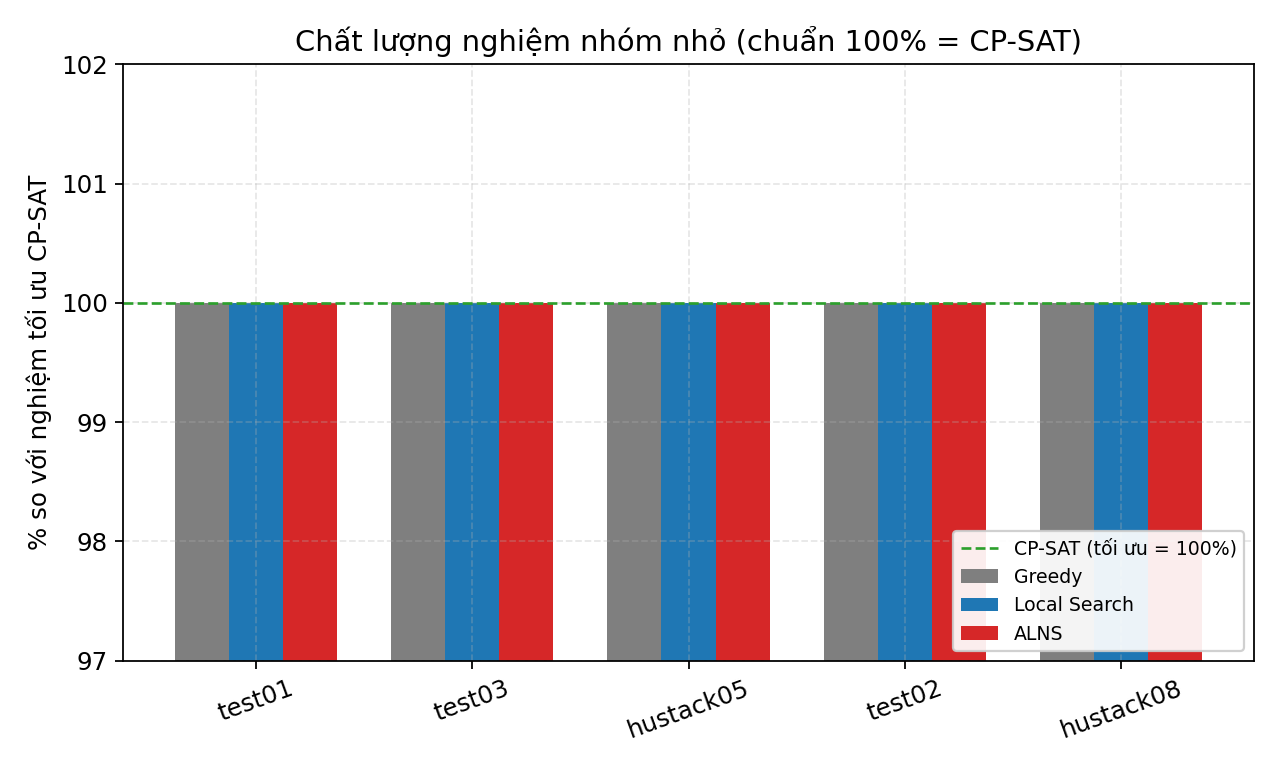
\includegraphics[width=\linewidth]{figures/bench_small_quality.png}
    \caption{Nhóm nhỏ: \% so với CP-SAT}
  \end{subfigure}\hfill
  \begin{subfigure}{0.49\textwidth}
    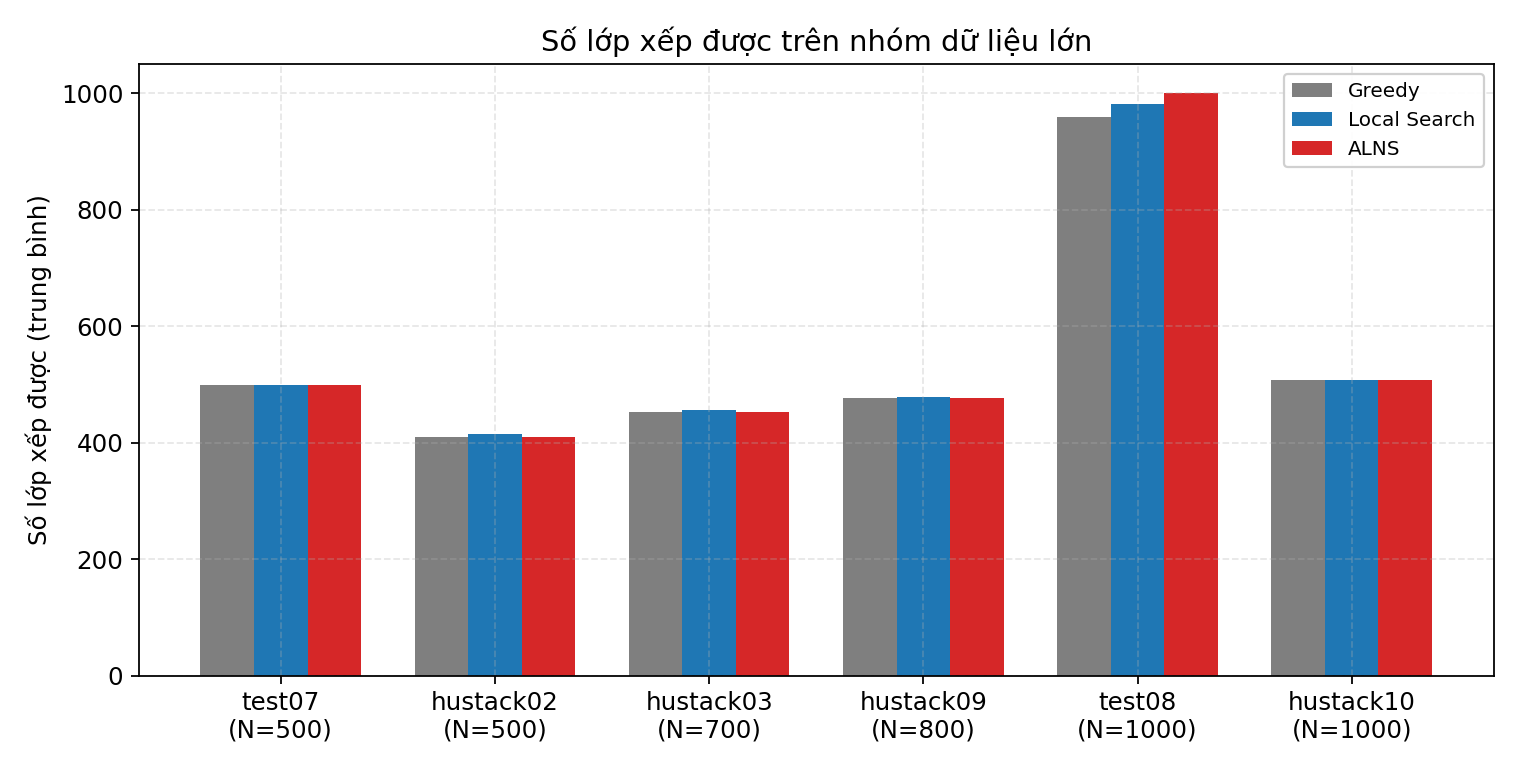
\includegraphics[width=\linewidth]{figures/bench_large_gain.png}
    \caption{Nhóm lớn: số lớp xếp được}
  \end{subfigure}
  \caption{Chất lượng nghiệm: nhóm nhỏ bám chuẩn tối ưu; nhóm lớn --- ALNS đạt tối
  ưu trên \texttt{test08} (còn khe cấu trúc lớn), còn trên các instance nghẽn HUStack
  thì LS nhỉnh hơn.}
  \label{fig:bench-quality}
\end{figure}

\begin{figure}[H]
  \centering
  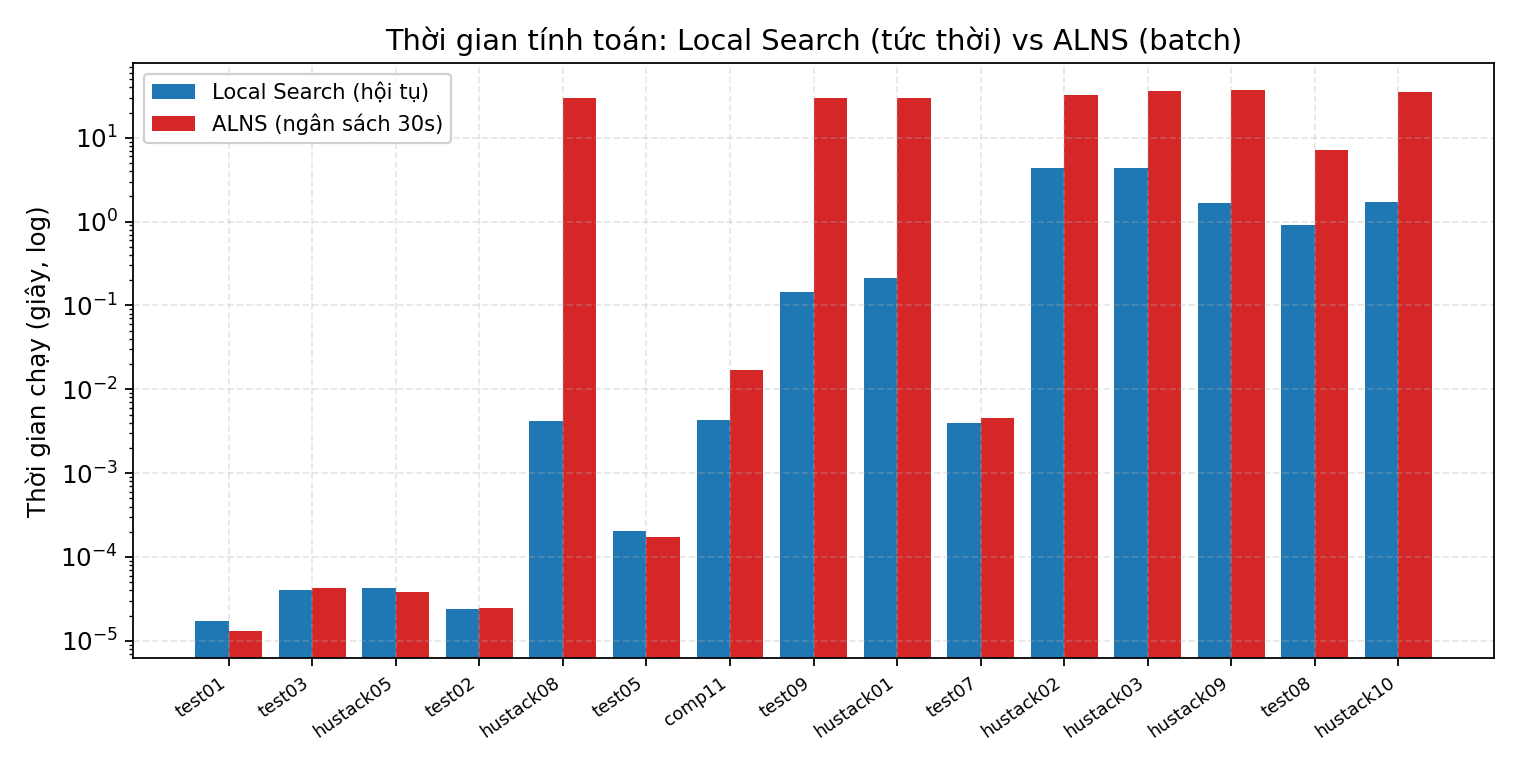
\includegraphics[width=0.82\textwidth]{figures/bench_runtime.png}
  \caption{Thời gian tính toán (thang log): Local Search hội tụ rất nhanh ---
  mili-giây trên dữ liệu nhỏ/thưa, tới vài giây trên instance lớn nghẽn (vd
  \texttt{hustack02} $\approx 4.4$s) --- vẫn nhanh hơn ALNS nhiều bậc; ALNS dùng
  trọn ngân sách $30$s trên instance nghẽn.}
  \label{fig:bench-runtime}
\end{figure}

\subsection{Phân tích và thảo luận}
\label{sec:discussion}
Giao thức công bằng (cùng ngân sách $30$s) cho ra bốn nhận định --- trong đó nhận
định thứ ba là một phát hiện đáng giá mà chỉ phép so sánh \emph{đồng thời gian} mới
bộc lộ.

\begin{enumerate}[leftmargin=*]
  \item \textbf{Quy mô nhỏ: heuristic là đủ.} Trên toàn nhóm nhỏ, Greedy, LS, ALNS
  đều đạt $100\%$ tối ưu CP-SAT (Bảng~\ref{tab:bench-small}). Thuật toán phức tạp ở
  đây là dư thừa.

  \item \textbf{Thuật toán Tham lam (Greedy best-fit) thu hẹp mạnh khoảng cách,
  nhưng vẫn còn dư địa.} Nhờ chiến lược sắp xếp ưu tiên (thời lượng tăng, sĩ số
  tăng) kết hợp với best-fit phòng (Mục~\ref{sec:init}), bản thân Greedy đã tiệm cận
  rất sát mức tối ưu trên các tập dữ liệu nghẽn lớn --- thậm chí đạt tối ưu tuyệt
  đối trên \texttt{hustack10} ($508$). Dù vậy, thuật toán vẫn để sót một số lượng
  nhỏ các lớp (\texttt{test09}: $125$, \texttt{test08}: $959$, \texttt{comp11}:
  $147$). Phần hao hụt này chính là không gian tối ưu dành cho các thuật toán
  LS/ALNS thể hiện.

  \item \textbf{Điểm giao thoa hiệu năng giữa LS và ALNS phụ thuộc vào đặc tính của
  dư địa cải thiện, không thuần túy do quy mô.}
  \begin{itemize}
    \item Khi hệ thống tồn tại các \emph{khoảng trống cấu trúc lớn} cần được tái sắp
    xếp, ALNS hoàn toàn áp đảo: trên \texttt{hustack01}, ALNS đạt $193.7$ so với LS
    $184.3$; trên \texttt{test08} ($N{=}1000$), ALNS vươn tới mức tối ưu tuyệt đối
    $1000$ trong khi LS mắc kẹt ở ``hiệu ứng cao nguyên'' với $982.5$. Cơ chế phá vỡ
    và tái tạo (ruin \& recreate) đã phát huy đúng kỳ vọng.
    \item Ngược lại, trên các tập dữ liệu thực tế có độ nghẽn cực cao của HUStack,
    LS lại chiến thắng: \texttt{hustack02} ($415.5$ vs $410.5$), \texttt{hustack03}
    ($455.5$ vs $453.0$), \texttt{hustack09} ($478.0$ vs $477.0$).
  \end{itemize}
  Nguyên nhân cốt lõi nằm ở \emph{chi phí tính toán của mỗi vòng lặp}. Toán tử
  Regret-2 của ALNS có độ phức tạp quét (lớp $\times$ phòng $\times$ tiết) nên chi
  phí tăng vọt theo $N$, khiến ALNS thực hiện được rất ít vòng lặp trong ngân sách
  $30$s. Trong khi đó, mỗi vòng lặp của LS tốn chi phí cực rẻ, tạo ra sự áp đảo về
  ``số vòng khám phá''. \textbf{Bài học rút ra:} dưới ràng buộc thời gian thực tế
  (time-limit), tốc độ thực thi của vòng lặp quan trọng ngang bằng với chất lượng
  của vòng lặp đó; không một phương pháp xấp xỉ nào là thống trị tuyệt đối --- điều
  này càng củng cố giá trị của kiến trúc hệ thống đa tầng có định tuyến.

  \item \textbf{Bộ giải chính xác không thống trị trong ngân sách.} Bức tranh trộn
  lẫn: CP-SAT đạt tối ưu trên \texttt{test09} ($131$), \texttt{hustack10} ($508$) và
  thậm chí \emph{dẫn đầu} trên \texttt{hustack01} ($196$, hơn mọi heuristic); nhưng
  trên \texttt{hustack02}/\texttt{hustack03} nó \emph{kẹt ngay mức Greedy}
  ($410, 453$) và thua LS, còn trên \texttt{test08} chỉ đạt \textsc{feasible} $990$
  --- kém ALNS ($1000$). Đây là minh chứng cho thiết kế đa tầng: ở quy mô nghẽn lớn,
  heuristic/metaheuristic trong cùng thời gian có thể cho nghiệm \emph{tốt hơn} bộ
  giải ``tối ưu''. Đánh đổi thời gian--chất lượng được định lượng ở
  Bảng~\ref{tab:tradeoff}.
\end{enumerate}

\begin{table}[H]
\centering\small
\caption{Đánh đổi thời gian--chất lượng: Local Search (hội tụ tự nhiên) so với
ALNS (ngân sách $30$s). $\Delta\%$ là chênh lệch số lớp của ALNS so với LS
(giá trị \emph{âm} nghĩa là LS tốt hơn, ví dụ \texttt{hustack02}).}
\label{tab:tradeoff}
\begin{tabular}{ll r rr rr r}
\toprule
Instance & Nhóm & $N$ & LS (ms) & ALNS (s) & LS avg & ALNS avg & $\Delta\%$ \\
\midrule
\texttt{test01} & small & 5 & 0.0 & 0.00 & 5.0 & 5.0 & +0.00\% \\
\texttt{test03} & small & 20 & 0.0 & 0.00 & 20.0 & 20.0 & +0.00\% \\
\texttt{hustack05} & small & 20 & 0.0 & 0.00 & 20.0 & 20.0 & +0.00\% \\
\texttt{test02} & small & 10 & 0.0 & 0.00 & 10.0 & 10.0 & +0.00\% \\
\texttt{hustack08} & small & 10 & 4.2 & 30.00 & 9.0 & 9.0 & +0.00\% \\
\texttt{test05} & medium & 100 & 0.2 & 0.00 & 100.0 & 100.0 & +0.00\% \\
\texttt{comp11} & medium & 162 & 4.3 & 0.02 & 162.0 & 162.0 & +0.00\% \\
\texttt{test09} & medium & 200 & 144.0 & 30.03 & 127.0 & 128.3 & +1.05\% \\
\texttt{hustack01} & medium & 200 & 212.6 & 30.02 & 184.3 & 193.7 & +5.06\% \\
\texttt{test07} & large & 500 & 4.0 & 0.00 & 500.0 & 500.0 & +0.00\% \\
\texttt{hustack02} & large & 500 & 4401.1 & 32.77 & 415.5 & 410.5 & -1.20\% \\
\texttt{hustack03} & large & 700 & 4414.5 & 36.12 & 455.5 & 453.0 & -0.55\% \\
\texttt{hustack09} & large & 800 & 1677.3 & 36.98 & 478.0 & 477.0 & -0.21\% \\
\texttt{test08} & large & 1000 & 908.3 & 7.08 & 982.5 & 1000.0 & +1.78\% \\
\texttt{hustack10} & large & 1000 & 1693.8 & 34.87 & 508.0 & 508.0 & +0.00\% \\
\bottomrule
\end{tabular}
\end{table}

